\documentclass[11pt,a4paper]{article}
\usepackage[inline]{enumitem}
\usepackage{amsfonts}
\usepackage{amsmath,amssymb,amsthm}
\usepackage{mathtools}
\usepackage{graphicx, subcaption}
\usepackage[margin=1in,a4paper]{geometry}
\usepackage{algorithm}
\usepackage{algorithmic}
% \usepackage[font= scriptsize]{subcaption}
\usepackage{xcolor}
\usepackage{natbib}
\usepackage{tabu}
\usepackage{multirow} 
\usepackage[colorlinks,citecolor=blue,urlcolor=blue,bookmarks=false,hypertexnames=true]{hyperref} 
%\usepackage[utf8]{inputenc}
\usepackage{newunicodechar}
\providecommand{\keywords}[1]{\noindent\textbf{{Keywords:}} #1}
\usepackage{rotating}

\usepackage{mathtools}
\usepackage{setspace}
\mathtoolsset{showonlyrefs=true}
\newtheorem{proposition}{Proposition}
\newtheorem{corollary}{Corollary}
\newtheorem{lemma}{Lemma}
\newtheorem{definition}{Definition}
\newtheorem{assumption}{Assumption}
\newtheorem{theorem}{Theorem}
\theoremstyle{remark}
\newtheorem{remark}{Remark}
\newtheorem{example}{Example}
\setlength{\bibsep}{0.0pt}
\allowdisplaybreaks[4]

\usepackage{todonotes}

\title{Hamiltonian Neural Network for Hamiltonian Monte Carlo}

\begin{document}

\maketitle

This paper explains the parts of \cite{dhulipala2023efficient} that are difficult to understand and presents the replication results obtained using TensorFlow.

\subsection{Typos and Explaination}
\begin{itemize}
	\item On page 9, the sentence \textit{"where $\{q^+, p^+\}$ and $\{q^-, p^-\}$ are, respectively, the leftmost and rightmost states of a sub-tree in the binary tree."} What do the leftmost and rightmost states mean in high dimensions? In high dimensions, the right direction corresponds to positive step size $dt$, while the left direction corresponds to negative step size $dt$.
    \item On page 9, what error does the equation (20) measure? The error monitors the integration error. According to the simulation method of $u$ in Algorithm 4, we know that $\log u + H(q(0), p(0)) < 0$. If the integration error is small, it should hold that $\log u + H(q, p) < \Delta_{\text{max}}$. Otherwise, if this inequality is violated, the integration error is very large, and the tree should stop.
    \item In line 16 of Algorithm 4, there is a typo. It should be $\nu_j$ instead of $j$.
    \item In Section 3.2, the author does not specify the activation function. In my implementation, I tried "sin", "ReLU", and "tanh". The loss did not decrease at all when using "ReLU," whereas both "sin" and "tanh" produced similar results.
    \item In Section 7.2, the author does not explicitly mention the target density. Therefore, we need to derive the target density for this elliptic PDE problem ourselves. Given that $u(x, y) = \sin(2x) + \sin(2y)$, the PDE can be written explicitly as:
\begin{align*}
    & \frac{\partial}{\partial x}\left(k(x, y) \frac{\partial u}{\partial x}\right) + \frac{\partial}{\partial y}\left(k(x, y) \frac{\partial u}{\partial y}\right) \\
    = & \frac{\partial k}{\partial x}(x, y) 2\cos 2x - k(x, y) 4\sin 2x + \frac{\partial k}{\partial y}(x, y) 2\cos 2y - k(x, y) 4\sin 2y.
\end{align*}
Let $\{(x_i, y_i), i = 1, \dots, 50\}$ denote the 50 sensor locations, and let $q, h \in \mathbb{R}^{50}$ represent the values of $k$ at these 50 locations (to be inferred) and the observations of $f$, respectively. The target density can be expressed as:
\begin{align}
    f(q) \propto & \exp\left( - \frac{1}{2} \sum_{i=1}^{50} \left( \hat{\frac{\partial k}{\partial x}}(x_i, y_i) 2\cos 2x_i - q_i 4\sin 2x_i \right.\right. \nonumber \\
    & \qquad \quad \left.\left. + \hat{\frac{\partial k}{\partial y}}(x_i, y_i) 2\cos 2y_i - q_i 4\sin 2y_i - h_i \right)^2 \right),
\end{align}
where $\hat{\frac{\partial k}{\partial x}}$ and $\hat{\frac{\partial k}{\partial y}}$ represent approximations of the partial derivatives. There are various methods to approximate these derivatives; here, we use a simple approach. Assume $k(x, y) = ax + by$. With 50 observations of $k$, the coefficients $(a, b)$ can be approximated using linear regression:
\begin{align}
    (\hat{a}, \hat{b}) = (X^T X)^{-1} X^T q,
\end{align}
where $X \in \mathbb{R}^{50 \times 2}$ is the matrix of stacked sensor values. Substituting these approximations, the target density becomes:
\begin{align}
    f(q) \propto & \exp\left( - \frac{1}{2} \sum_{i=1}^{50} \left( \hat{a} 2\cos 2x_i - q_i 4\sin 2x_i + \hat{b} 2\cos 2y_i - q_i 4\sin 2y_i - h_i \right)^2 \right).
\end{align}
\end{itemize}

\subsection{Replication Results}
I used TensorFlow to replicate the results presented in \cite{dhulipala2023efficient}. All the figures and tables referenced in this subsection are available in the file "plot\_Dhulipapa.ipynb".

\smallskip 
\noindent \textbf{Sampling under 1D Gaussian mixture} I used "sin" as the activation function and tested the L-HNN for HMC on the 1D Gaussian mixture model. The phase space plot and sample histograms are presented in Figure \ref{fig:fig2}, while the time reversibility and Hamiltonian conservation plots are shown in Figure \ref{fig:fig3}. These figures demonstrate that my trained HNN performs comparably to the trained HNN in \cite{dhulipala2023efficient} on the 1D Gaussian mixture model.

\begin{figure}
\centering
\subcaptionbox{\label{fig:2a}}{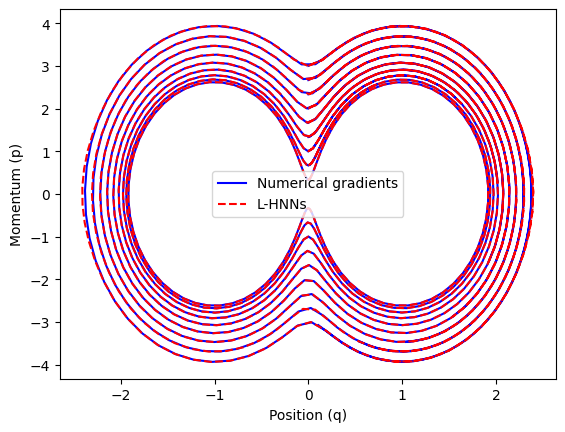
\includegraphics[width=0.3\textwidth]{../figures/fig2a.png}}
\subcaptionbox{\label{fig:2b}}{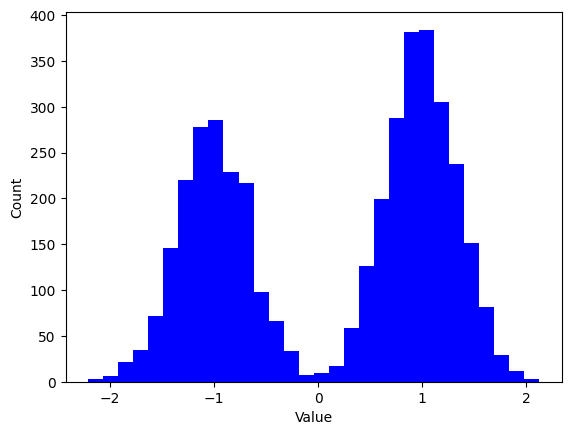
\includegraphics[width=0.3\textwidth]{../figures/fig2b.png}}
\subcaptionbox{\label{fig:2c}}{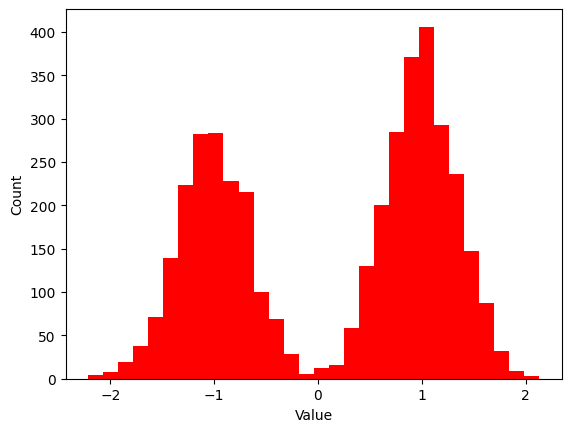
\includegraphics[width=0.3\textwidth]{../figures/fig2c.png}}
\caption{(a) \{q,p\}phase space plot corresponding to different energy levels. (b) and (c) Histogram of samples from a 1-D Gaussian mixture density using traditional HMC and L-HNNs in HMC, respectively.}
\label{fig:fig2}
\end{figure}

\begin{figure}
\centering
\subcaptionbox{\label{fig:3a}}{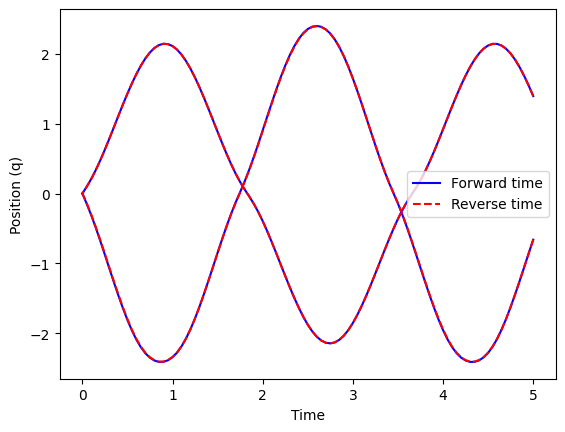
\includegraphics[width=0.3\textwidth]{../figures/fig3a.png}}
\quad 
\subcaptionbox{\label{fig:3b}}{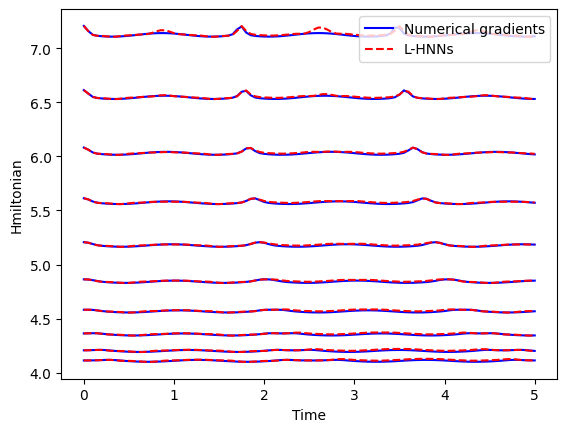
\includegraphics[width=0.3\textwidth]{../figures/fig3b.png}}
\caption{(a) Time reversibility of the L-HNNs in predicting the Hamiltonian dynamics under two different
sets of initial conditions, given a 1-D Gaussian mixture density. (b) Conservation of the Hamiltonian for
different energy levels given a 1-D Gaussian mixture density.}
\label{fig:fig3}
\end{figure}


\smallskip 
\noindent \textbf{NUTS with L-HNNs} Table \ref{tab:tab1} shows that our trained model performs similarly to \cite{dhulipala2023efficient}. Under both HMC and NUTS, the ESS has significantly improved, and the improvement percentage is comparable to that reported in \cite{dhulipala2023efficient}. From Figure \ref{fig:fig4}, I observed some degeneracy in the path; however, it was not as pronounced as that reported in \cite{dhulipala2023efficient}. This difference could be attributed to randomness, as well as the possibility that they used a less well-trained HNN to intentionally demonstrate stronger degeneracy.

\begin{table}
\caption{Comparison of the performance of traditional HMC, traditional NUTS, HNN-HMC, and HNNNUTS, considering a 1-D Gaussian mixture density. ESS per gradient is used as the performance metric.}
\label{tab:tab1}
\centering
	\begin{tabular}{|c|c|}
\hline & \begin{tabular}{c}
ESS per gradient \\
of target density
\end{tabular} \\
\hline L-HNNs in HMC & $5.87 E-3$ \\
\hline Traditional HMC & $9.30 E-5$ \\
\hline L-HNNs in NUTS & $4.02 E-3$ \\
\hline Traditional NUTS & $4.03 E-4$ \\
\hline
\end{tabular}
\end{table}

\begin{figure}
\centering
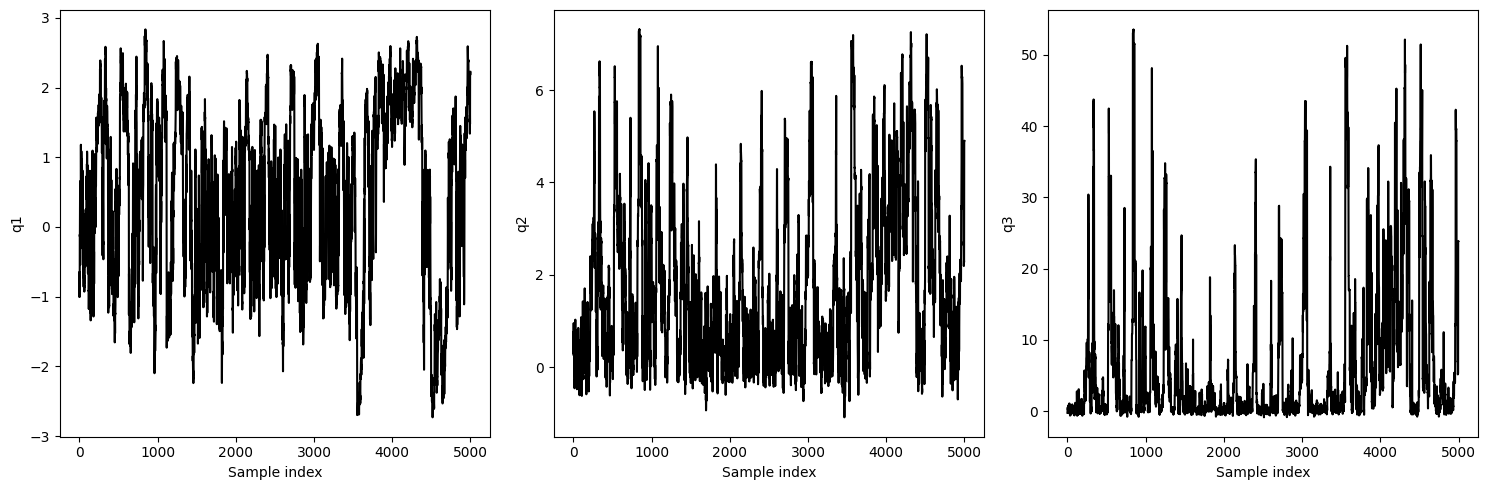
\includegraphics[width=0.9\textwidth]{../figures/fig4.png}
\caption{Degeneracy in sampling when using L-HNNs in NUTS for a 3-D Rosenbrock density. These trace
plots correspond to the three dimensions q1, q2, and q3.}
\label{fig:fig4}
\end{figure}


\smallskip 
\noindent \textbf{Sampling from a 3-D Rosenbrock density} Figure \ref{fig:fig5} is similar to that in \cite{dhulipala2023efficient}. Figure \ref{fig:fig6} shows that the integration error of L-HNN is generally smaller than that of HNN; however, the difference is not as significant as reported in \cite{dhulipala2023efficient}. In fact, I believe there is no real difference between L-HNN and HNN. According to the L-HNN formula (Equation (16) in \cite{dhulipala2023efficient}), given $\mathbf{u}_P$ as the output of a $P$-layer neural network, and $\mathbf{\omega}_P$ and $\mathbf{b}_P$ as the weights and biases, the L-HNN is defined as:
\begin{equation}
    H_\theta = \mathbf{1}^T \mathbf{\lambda} = \mathbf{1}^T (\mathbf{\omega}_P \mathbf{u}_P + \mathbf{b}_P) = \mathbf{1}^T \mathbf{\omega}_P \mathbf{u}_P + \mathbf{1}^T \mathbf{b}_P,
\end{equation}
which is mathematically equivalent to an HNN with $\mathbf{1}^T \mathbf{\omega}_P$ and $\mathbf{1}^T \mathbf{b}_P$ as the weights and biases of the last layer. Therefore, I believe that Figure 6 in \cite{dhulipala2023efficient} presents an unfair comparison. Figure \ref{fig:fig7} and Table \ref{tab:tab2} are similar to that in \cite{dhulipala2023efficient}.

\begin{figure}
\centering
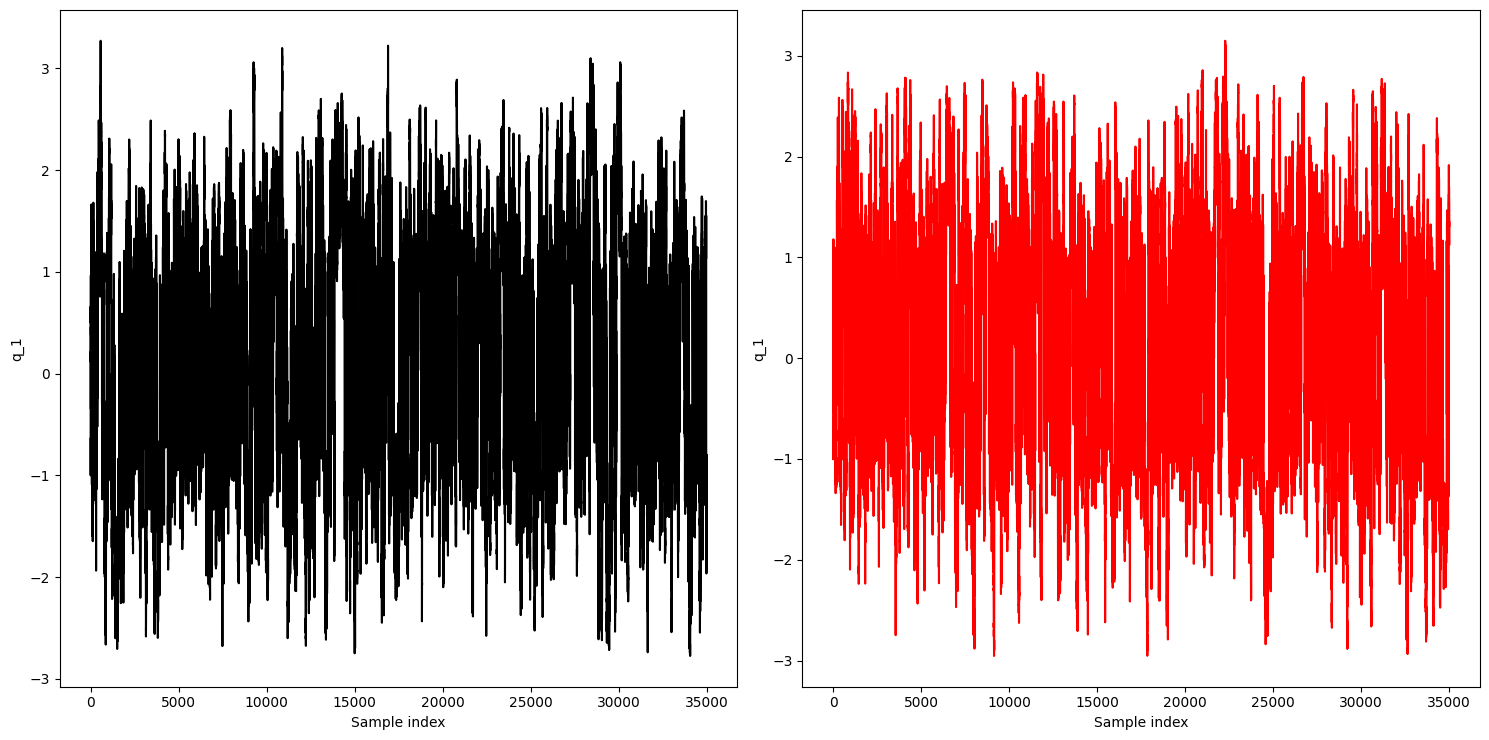
\includegraphics[width=0.7\textwidth]{../figures/fig5.png}
\caption{Trace plots of dimension q1 for a 3-D Rosenbrock density simulated via efficient NUTS with online error monitoring using (left) HNNs and (right) L-HNNs.}
\label{fig:fig5}
\end{figure}

\begin{figure}
\centering
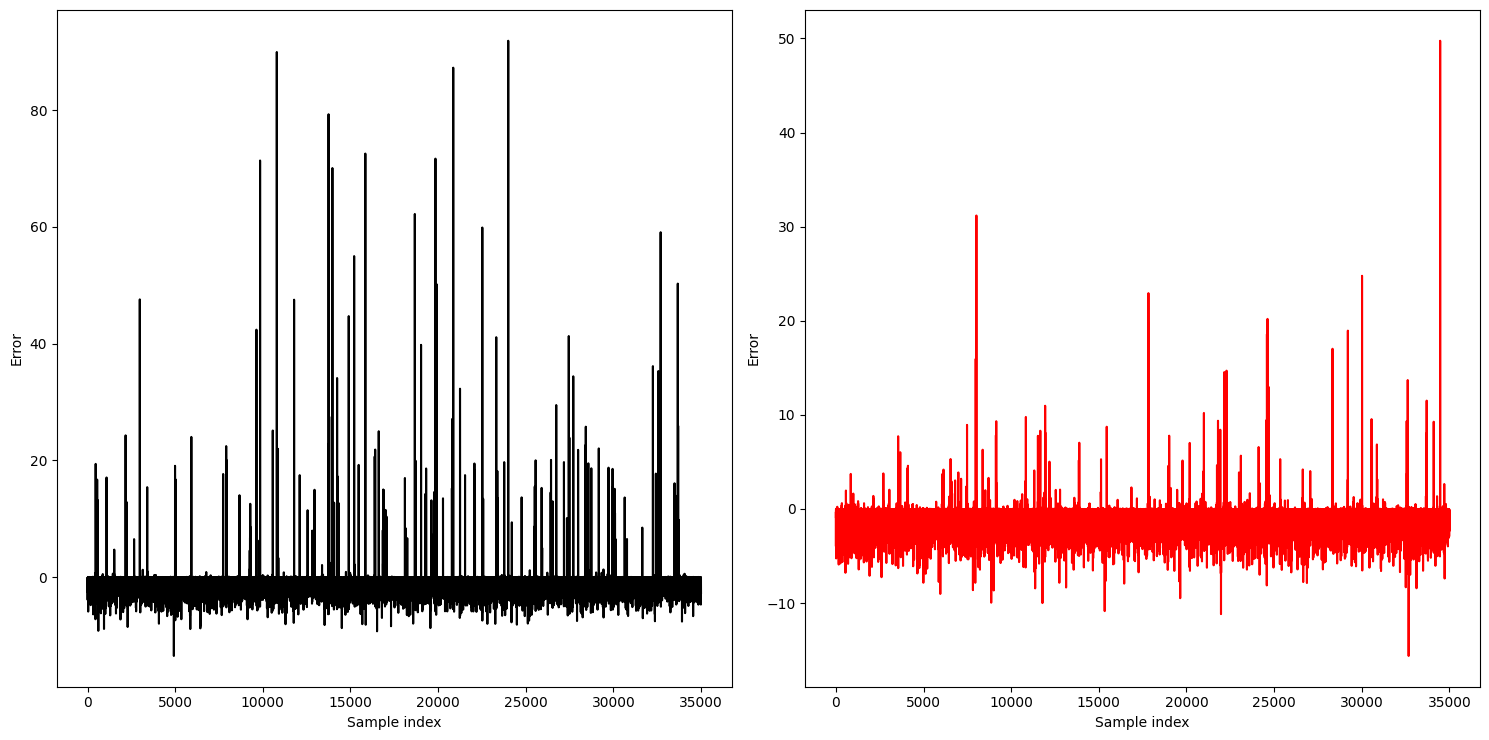
\includegraphics[width=0.7\textwidth]{../figures/fig6.png}
\caption{L-HNNs error metric, as defined by the quantity $\varepsilon \equiv H(q', p') + \log u$ in Algorithm 5, while generating samples from a 3-D Rosenbrock density using (left) HNNs and (right) L-HNNs in efficient NUTS with online error monitoring.}
\label{fig:fig6}
\end{figure}


\begin{figure}
\centering
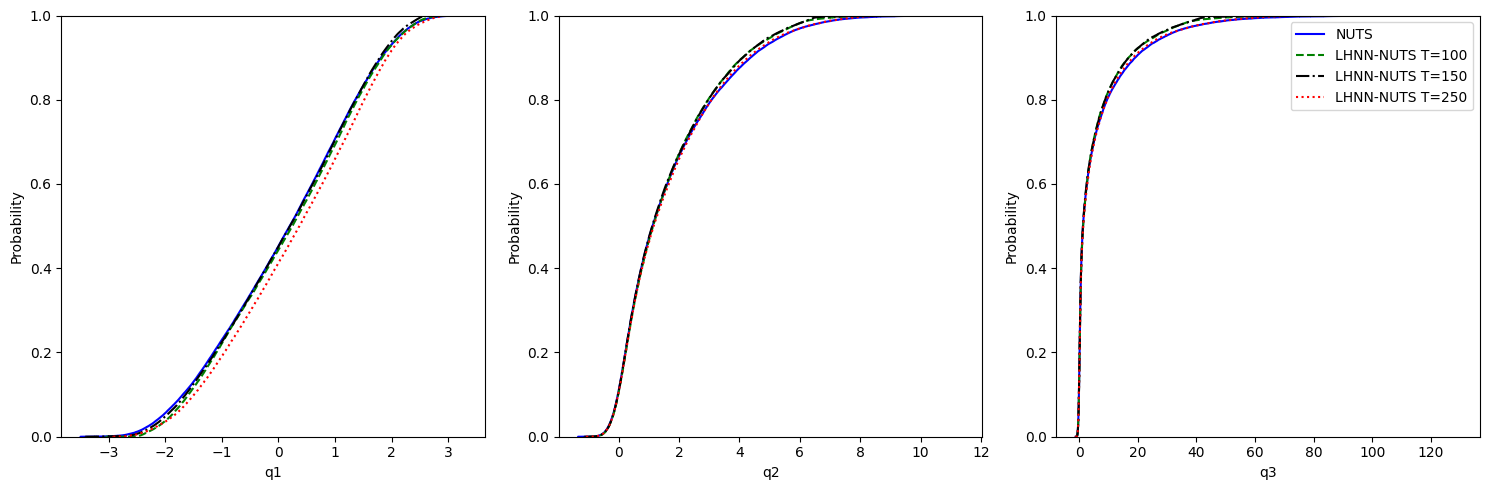
\includegraphics[width=0.9\textwidth]{../figures/fig7.png}
\caption{Empirical CDF plots of samples from a 3-D Rosenbrock density simulated via NUTS and L-HNNs
in NUTS with online error monitoring, using different training datasets. eCDF plots are presented for the dimensions q1, q2, and q3. }
\label{fig:fig7}
\end{figure}


\begin{table}[h!]
\centering
\caption{Performance comparison between traditional NUTS and HNN-NUTS with different training data characteristics, considering a 3-D degenerate Rosenbrock density.}
\label{tab:tab2}
\resizebox{0.9\textwidth}{!}{
\begin{tabular}{|c|c|c|c|}
\hline
 & ESS & \begin{tabular}{c}
 	\# gradients of \\ target density
 \end{tabular}  & \begin{tabular}{c}
 	Avg. ESS per \\ 
 	gradient of \\ 
 	target density 
 \end{tabular}\\
\hline
NUTS & 
\begin{tabular}{c}
(1306.86, 1968.87, \\ 
2074.03)
\end{tabular} & 
13,004,142 & 
0.000137 \\
\hline
\begin{tabular}{c}
$M_t = 40$, $T = 100$ \\ 
LHNN-NUTS 1
\end{tabular} & 
\begin{tabular}{c}
(1509.69, 2355.79,\\ 1962.16)
\end{tabular} & 
\begin{tabular}{c}
1,105,447 \\ 
Training: 160,000 \\ 
Evaluation: 945,447
\end{tabular} & 
0.001757 \\
\hline
\begin{tabular}{c}
$M_t = 40$, $T = 150$ \\ 
LHNN-NUTS 2
\end{tabular} & 
\begin{tabular}{c}
(1378.65, 2084.02 \\ 1990.07)
\end{tabular} & 
\begin{tabular}{c}
837,691\\
Training: 240,000 \\ 
Evaluation: 597,691
\end{tabular} & 
0.002170 \\
\hline
\begin{tabular}{c}
$M_t = 40$, $T = 250$ \\ 
LHNN-NUTS 3
\end{tabular} & 
\begin{tabular}{c}
(1547.13, 2156.33,\\ 2327.47)
\end{tabular} & 
\begin{tabular}{c}
413,840 \\ 
Training: 400,000 \\ 
Evaluation: 13,840
\end{tabular} & 
0.004858 \\
\hline
\end{tabular}
}
\label{tab:performance_comparison}
\end{table}


\smallskip
\noindent \textbf{Analytical case studies.} It is worth mentioning that Dhulipala had a typo in the density function of the 2-D Neal’s funnel density. The variance of $q_1$ should be $3^2 = 9$. Therefore, the correct 2-D Neal’s funnel density should be defined as:
\begin{align*}
&f(\boldsymbol{q}) \propto\left\{\begin{array}{l}
q_1=\mathcal{N}(0,9) \\
q_2=\mathcal{N}\left(0, \exp ^{q_1}\right)
\end{array}\right. .
\end{align*}
In the implementation, the correct density is used. L-HNNs are trained on a sampling of the 2-D Neal’s funnel density, the 5-D ill-conditioned Gaussian density, and the 10-D degenerate Rosenbrock density. Table \ref{tab:tab3} and Figures \ref{fig:fig9} and \ref{fig:fig10} show results similar to those reported in \cite{dhulipala2023efficient}. 


\begin{figure}
\centering
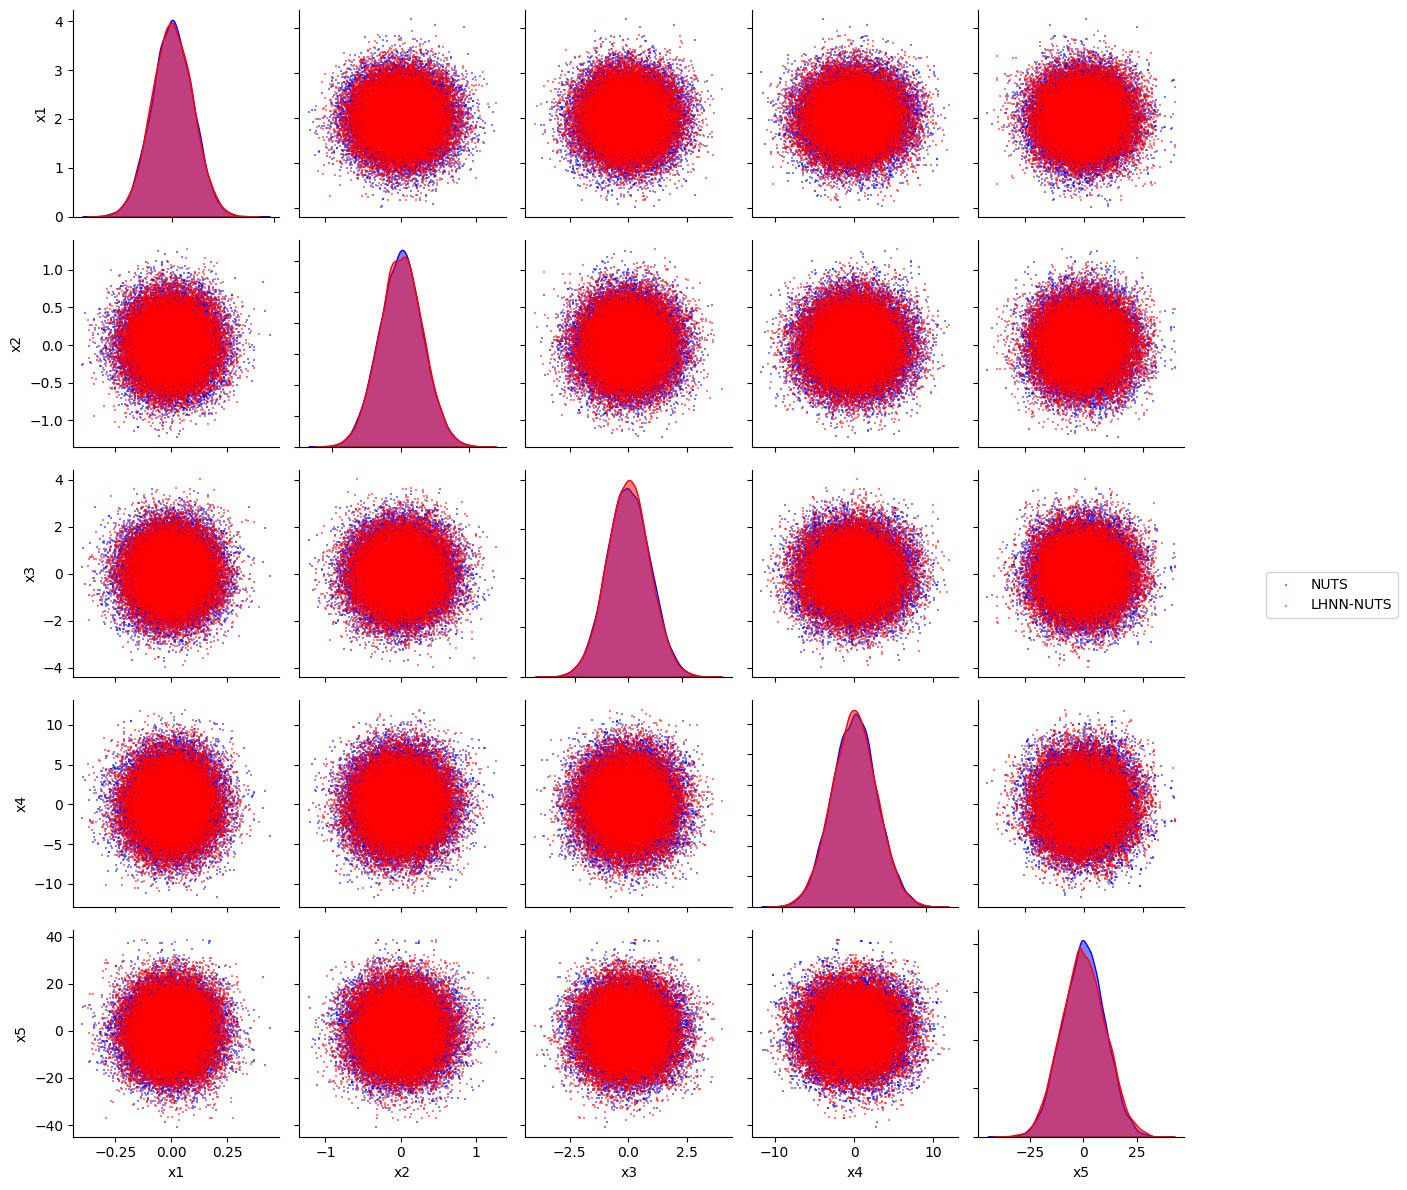
\includegraphics[width=0.9\textwidth]{../figures/fig9.png}
\caption{Scatter plot comparison between NUTS and LHNN-NUTS with online error monitoring for a 5-D ill-conditioned Gaussian distribution. (Blue dots: traditional NUTS; Red dots: LHNN-NUTS with online
error monitoring)}
\label{fig:fig9}
\end{figure}

\begin{figure}
\centering
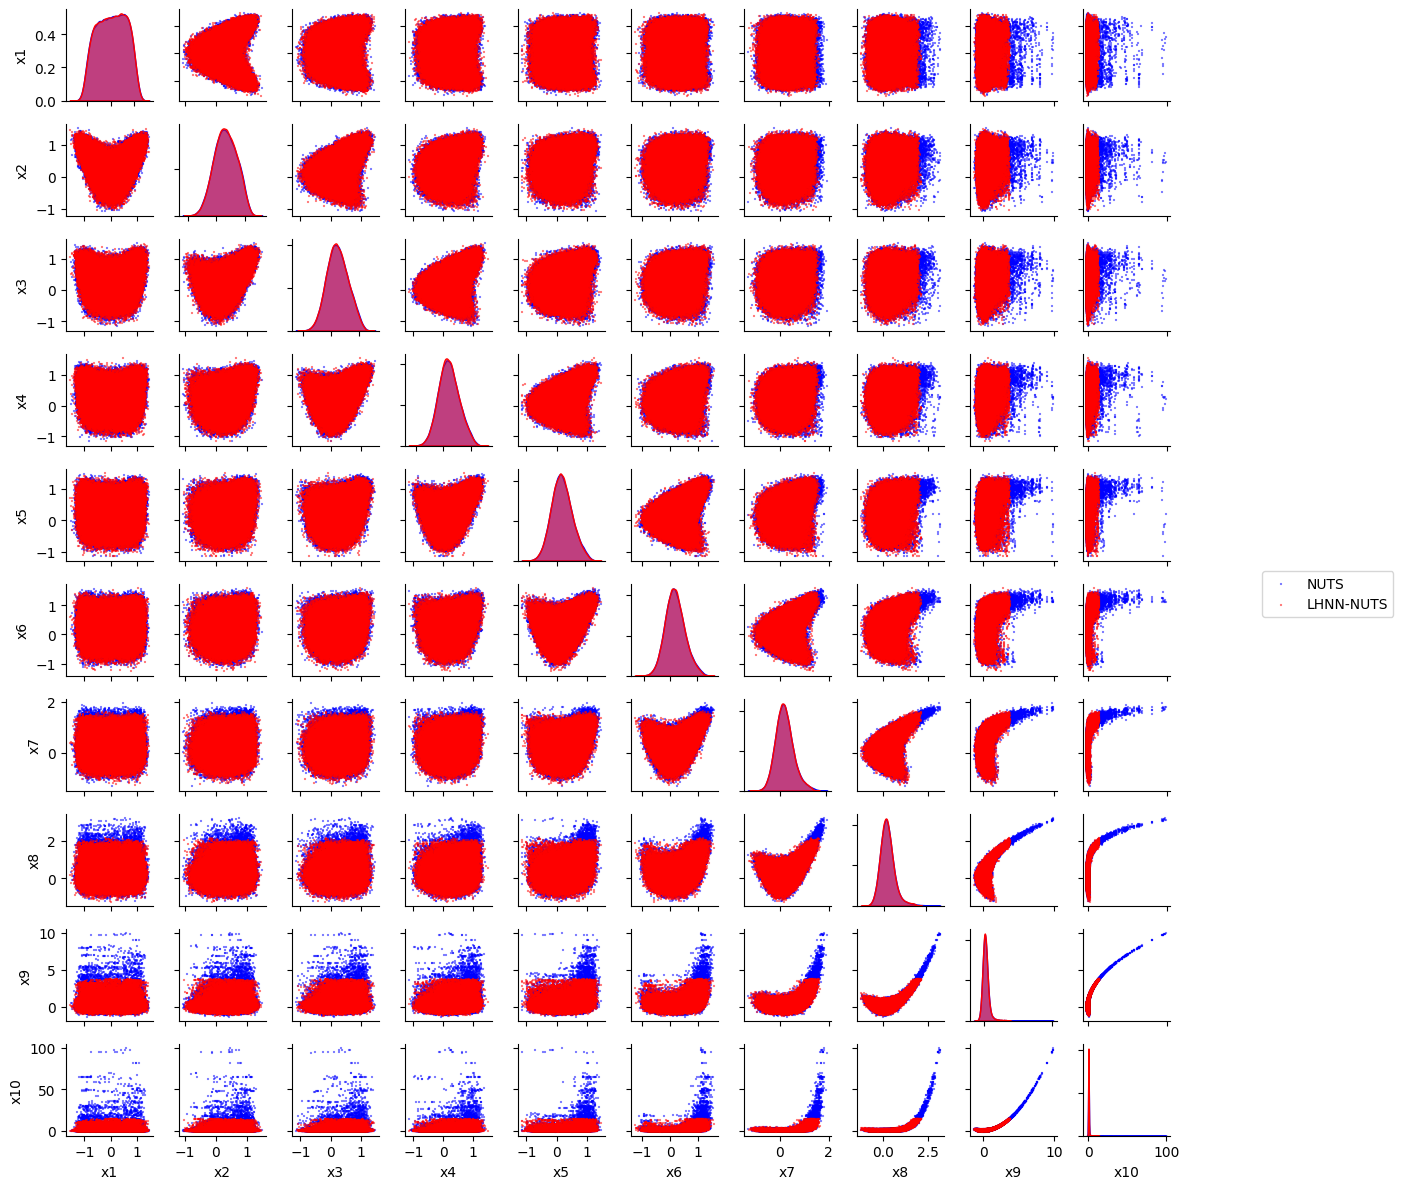
\includegraphics[width=0.9\textwidth]{../figures/fig10.png}
\caption{Scatter plot comparison between NUTS and LHNN-NUTS with online error monitoring, considering a 10-D degenerate Rosenbrock distribution. (Blue dots: traditional NUTS; Red dots: LHNN-NUTS with online error monitoring)}
\label{fig:fig10}
\end{figure}


\begin{table}[h!]
\centering
\caption{Summary of the performance of LHNN-NUTS with online error monitoring across the different analytical case studies.}
\label{tab:tab3}
\resizebox{0.9\textwidth}{!}{ % Adjust the width to \textwidth
\begin{tabular}{|c|c|c|c|}
\hline
& ESS & \# gradients of target density & Avg. ESS per gradient of target density \\
\hline
\multicolumn{4}{|c|}{\textbf{2-D Neal’s funnel}} \\
\hline
LHNN-NUTS & 
\begin{tabular}{c} 
() 
\end{tabular} & 
\begin{tabular}{c} 
 \\ 
Training: 400,000 \\ 
Evaluation: 
\end{tabular} & 
 \\
\hline
NUTS & 
\begin{tabular}{c} 
(697.86, 503.90)
\end{tabular} & 
 13,625,586 & 0.000044
 \\
\hline
\multicolumn{4}{|c|}{\textbf{5-D ill-conditioned Gaussian}} \\
\hline
LHNN-NUTS & 
\begin{tabular}{c} 
(20000.02, 18144.69, \\ 14207.53, 8023.24,\\ 2472.59) 
\end{tabular} & 
\begin{tabular}{c} 
425,000 \\ 
Training: 400,000 \\ 
Evaluation: 25,000 
\end{tabular} & 
0.0295 \\
\hline
NUTS & 
\begin{tabular}{c} 
(20000, 17903.15,\\ 14658.81, 8185.42,\\ 2756.69) 
\end{tabular} & 
9,133,676 & 
0.00139 \\
\hline
\multicolumn{4}{|c|}{\textbf{10-D degenerate Rosenbrock}} \\
\hline
LHNN-NUTS & 
\begin{tabular}{c} 
(15447.20, 29445.31,\\ 27893.89, 25361.00,\\ 21654.22, 13608.50\\ 8473.87, 5864.44\\ 3544.28, 2039.00) 
\end{tabular} & 
\begin{tabular}{c} 
400,000 \\ 
Training: 400,000 \\ 
Evaluation: 0 
\end{tabular} & 
0.0383 \\
\hline
NUTS & 
\begin{tabular}{c} 
(15951.39, 27579.14,\\ 23974.31, 19612.90,\\ 13089.86, 8263.75,\\ 5217.63, 3198.49,\\ 1654.23, 1227.98) 
\end{tabular} & 
6,761,660 & 
0.00177 \\
\hline
\end{tabular}
}
\label{tab:summary_performance}
\end{table}

\smallskip
\noindent \textbf{Computational case studies} Table \ref{tab:tab4} and Figure \ref{fig:fig11} demonstrate that our results are consistent with those reported in \cite{dhulipala2023efficient}.

\begin{table}[h!]
\centering
\caption{Summary of the performance of LHNN-NUTS with online error monitoring across the different computational case studies.}
\label{tab:tab4}
\begin{tabular}{|c|c|c|c|}
\hline
 & ESS & \begin{tabular}{c}
 	\# gradients of \\ target density
 \end{tabular}  & \begin{tabular}{c}
 	Avg. ESS per \\ gradient of \\ target density
 \end{tabular}  \\
\hline
\multicolumn{4}{|c|}{\textbf{Allen-Cahn stochastic PDE (25 inference parameters)}} \\
\hline
LHNN-NUTS & 289 & 
\begin{tabular}{c}
7,272 \\ 
Training: 10,000 \\ 
Evaluation: 17,272 
\end{tabular} & 
0.016736 \\
\hline
NUTS & 232.42 & 581,752 & 0.00040 \\
\hline
\multicolumn{4}{|c|}{\textbf{Elliptic PDE (50 inference parameters)}} \\
\hline
LHNN-NUTS &  & 
\begin{tabular}{c}
 \\ 
Training: 64,000 \\ 
Evaluation:  
\end{tabular} & 
 \\
\hline
NUTS &  &  &  \\
\hline
\end{tabular}
\label{tab:performance_summary}
\end{table}

\begin{figure}
\centering
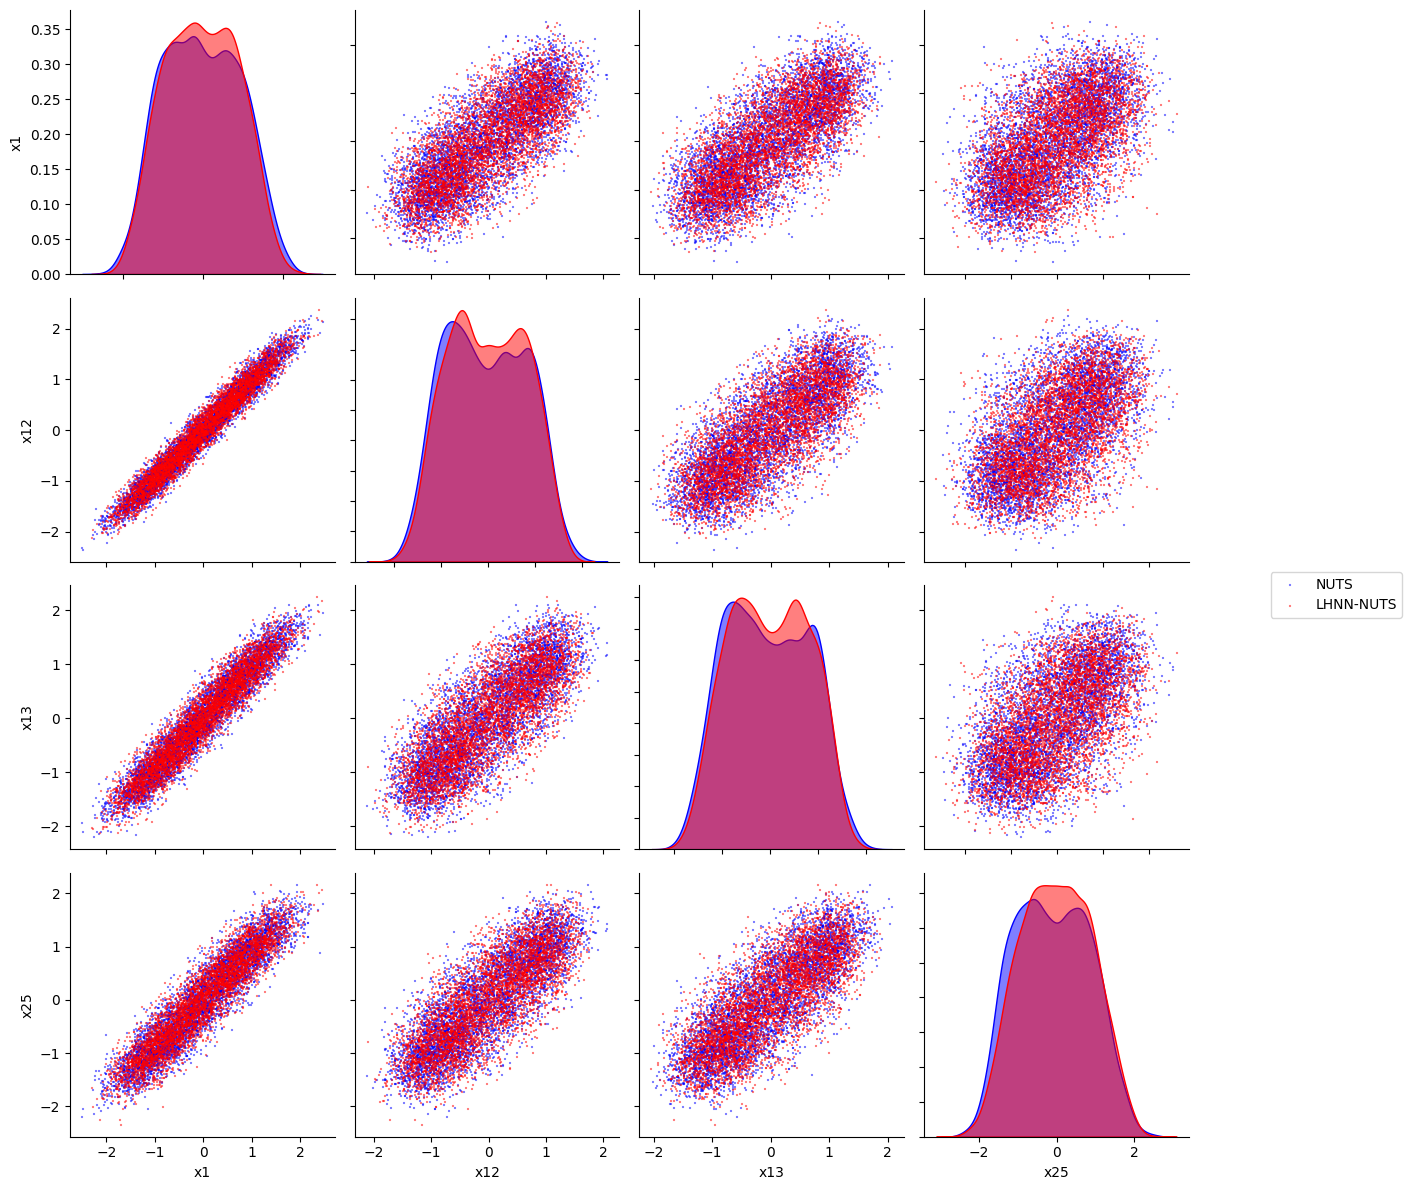
\includegraphics[width=0.9\textwidth]{../figures/fig11.png}
\caption{Sampling results for four of the 25 dimensions, namely, 1, 12, 13, and 25, of the Allen-Cahn equation. It is observed that the LHNN-NUTS and traditional NUTS results compare well with each other.}
\label{fig:fig11}
\end{figure}



\bibliographystyle{chicagoa}
\bibliography{refs}

\end{document}